\documentclass[tikz,border=3mm]{standalone}
\usetikzlibrary{calc,patterns}

\begin{document}
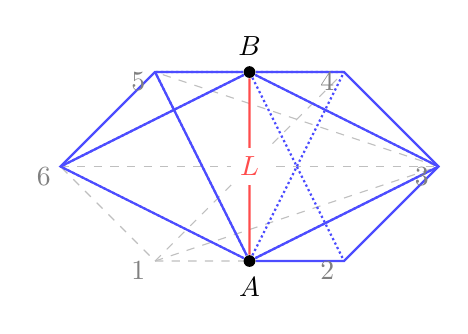
\begin{tikzpicture}[scale=1.2,
    original/.style={dashed,gray!50},
    new/.style={thick,blue!70},
    cut/.style={thick,red!70},
    vertex/.style={circle,fill,inner sep=1.5pt}
]

% Original polygon vertices
\coordinate (C1) at (0,0);
\coordinate (C2) at (2,0);
\coordinate (C3) at (3,1);
\coordinate (C4) at (2,2);
\coordinate (C5) at (0,2);
\coordinate (C6) at (-1,1);

% Original triangulation (dashed gray)
\draw[original] (C1) -- (C2) -- (C3) -- (C4) -- (C5) -- (C6) -- cycle;
\draw[original] (C1) -- (C3);
\draw[original] (C1) -- (C4);
\draw[original] (C3) -- (C5);
\draw[original] (C6) -- (C3);

% Define intersection points A and B
\node[vertex,label=below:$A$] (A) at (1,0) {};
\node[vertex,label=above:$B$] (B) at (1,2) {};

% Cutting line L
\draw[cut] (A) -- (B) node[midway,fill=white] {$L$};

% Remaining polygon edges after cutting
\draw[new] (A) -- (C2) -- (C3) -- (C4) -- (B);
\draw[new] (A) -- (C6) -- (C5) -- (B);
\draw[new] (A) -- (C3);
\draw[new] (A) -- (C5);
\draw[new] (B) -- (C3);
\draw[new] (B) -- (C6);

% New triangulation from A and B
\foreach \i in {C2,C3,C4,C5,C6} {
    \draw[new,densely dotted] (A) -- (\i);
    \draw[new,densely dotted] (B) -- (\i);
}

% Label original vertices
\foreach \c/\l in {C1/1,C2/2,C3/3,C4/4,C5/5,C6/6} {
    \node at (\c) [anchor=30,gray] {\l};
}

\end{tikzpicture}
\end{document}